\graphicspath{{chapters/02/images/}}
\chapter{Stochastic simulation of biochemical reaction systems}

\section{Introduction}
Biochemical reaction network can be modelled through stochastic chemical kinetics.
In this type of models the discreteness in population of species and the randomness of reactions are treated as an intrinsic part.
The dynamical behaviour is described by the chemical master equation or CME.

\section{Stochastic chemical kinetics}

  \subsection{Rewriting biochemical reactions}
  Biochemical reactions are the building blocks to model biological systems.
  They provide a unifying notation with sufficient level of details to represent complex biological processes.
  Biochemical reactions decorated with reaction kinetics can be simulated by a simulation algorithm to generate a realization of their dynamics.
  Chemical species in a biological system move around and gain kinetic energy.
  Upon collisions with other species, they undergo reactions to modify and transform into different species.

    \subsubsection{Representing molecular reactions}
    Molecular reactions can be classified between elementary reactions and non-elementary ones.
    The former require one step to complete, while the latter require a higher order reactions or a multi-step one.

      \paragraph{Some elementary reactions}

        \subparagraph{Unimolecolar reaction}
        An unimolecolar reaction involves the transformation of one species into another.
        It can be represented as:

        $$A\rightarrow B$$

        \subparagraph{Degradation}
        The degradation of a species is a special type of an unimolecolar reaction in which a species is degradated:

        $$A\rightarrow\emptyset$$

        Where the symbol $\emptyset$ represents a species that is not considered in the model, probably because it is large and does not change over time.

        \subparagraph{Synthesis}
        The synthesis of a species is another type of unimolecolar reaction in which a species is synthesised:

        $$\emptyset\rightarrow A$$

        This reaction is used to model the effects of the outside environment on system dynamics.

        \subparagraph{Bimolecular reaction}
        An example of a bimolecular reaction is an association reaction, in which a molecule can associated with another to produce a complex:

        $$A+B\rightarrow C$$

        Often this process is reversible and the inverse dissociation reaction can take place:

        $$A+B\xleftrightharpoons[]{} C$$

        \subparagraph{Dimerization}
        The dimerization is a special bimolecular reaction in which two molecules of the same species are consumed to produce another species:

        $$2A\rightarrow B$$

      \paragraph{Some non-elementary reactions}

        \subparagraph{Termolecular reaction}
        The thermolecular reaction is used to represent the polymerization of three molecules into another species.
        The original molecules can be of the same species:

        $$3A\rightarrow B$$

        Or of two different species:

        $$2A +B\rightarrow C$$

        \subparagraph{Enzymatic reaction}
        Another multi-step reaction is an enzymatic reaction, where the enzyme $W$ that catalyses the rate of conversion is kept the same:

        $$A+E\rightarrow B+E$$

    \subsubsection{Equation-based methods}
    The previous way to represent reactions does not give insight on the function of the equation.
    To shine light on this aspect equation-based methods need to be applied, like ordinary differential equation systems.
    In these the derivative with respect to time is specified for any of the variables in term of a function of the state.
    It can be noted how the stochastic simulation approach can be approximated by a deterministic one.

    \subsubsection{Creating a formal mathematical description of a biological system}
    To write a mathematical description of a biological system there is a need to:

    \begin{enumerate}
      \item Choose the biochemical reactions' representation.
      \item Choose the type of variable to describe the state of the system.
      \item Specify the likelihood of execution for each reaction.
    \end{enumerate}

    A reaction will be faster when there is a huge amount of reactants.
    This is because in term of probability: the more a species is present, the more it is likely to interact and for the reaction is to happen.
    This is true only when the assumption of that there is a well-mixed reaction volume is made.
    This assumption entails that the distribution of molecules is uniform.
    Moreover, in order to approximate a complex system the main compartments can be partitioned in smaller sets where a discretization procedure can be applied.
    Therefore in this case Petri nets are a suitable representation for these kind of systems.

    \subsubsection{Well-mixed reaction volume}
    A well-mixed reaction volume is a reaction volume in which all the molecular species are homogeneously distributed and spatially indistinguishable.
    The biochemical reaction system with well-mixed volume thus satisfies the spatial homogeneity condition, where spatial distribution of molecular species can be ignored.
    Chemical species under the well-mixed assumption at a thermal equilibrium are uniformly distributed in the volume $V$ and their velocities are thermally randomized according to the Maxwell-Boltzmann distribution.

    \subsubsection{Formal representation}
    The state of a spatially homogeneous biological system is determined by the population of each species, while the position and velocity of each individual molecule are ignored.
    Let $X_i(t)$ be the population of species $S_i$ at a particular time $t$.
    The N- vector $X(t) = (X_1(t),...,X_N(t))$, which determines the population of each species, constitutes the system state at the time $t$.
    A general reaction $R_j$ has a general scheme:

    $$v^-_{j1}S_1+...+v^-_{jN}S_N \rightarrow v^+_{j1}S_1+...+v^-_{jN}S_N$$

    Where:

    \begin{multicols}{2}
      \begin{itemize}
        \item Species on the left side are reactants.
        \item Species on the right side are products.
        \item The non-negative integers $v^-_{ji}$ and $v^+_{ji}$ are the stoichiometric coefficients which denote the number of molecules of a reactant that are consumed and the number of molecules of a product that are produced.
      \end{itemize}
    \end{multicols}

    For each reaction $R_j$, the net change in the population of species $S_i$ involved in the reaction is equal to $v^+_{ji}- v^-_{ji}$, which can be positive, negative or zero.
    The net changes by all reactions are described by a stoichiometry matrix $\mathbf{v}$ of size $M × N$.
    The \emph{j}th row $\mathbf{v}_j$ of the stoichiometry matrix expresses the changes caused by reaction $R_j$ and it is called the state change vector.
    Different system can lead to the same stoichiometric matrix.

    \subsubsection{Stoichiometric matrix}
    To describe a reaction two matrices are required:

    \begin{multicols}{2}
      \begin{itemize}
        \item $V^+$ provides the products.
        \item $V^-$ provides the reactants.
      \end{itemize}
    \end{multicols}

    $$ V^- = \begin{bmatrix}1 & 1 & 0 \\ 0 & 1&1 \\ 1&0&1 \end{bmatrix}, V^+ = \begin{bmatrix}0 & 2 & 0 \\ 0 & 0&2 \\ 2&0&0 \end{bmatrix}, V = \begin{bmatrix}1 & 1 & 0 \\ 0 & -1&1 \\ 1&0&-1 \end{bmatrix}\\ V = V^+ + V^- $$

    Suppose that at a time $t$ the state, or number of molecules in that given moment is $X(t)$.
    It is further assumed that the next reaction scheduled to fire at the next time $t + \tau$ is $R _\mu$, mill move the system accordingly to a new state $X(t + \tau)$.
    $\mathbf{x}$ is a simple notation to represent $X(t)$.
    So the evolution of the system in a time step will be:

    $$ X(t+\tau) = X(t)+v_\mu $$

    \subsubsection{Summary}
    While specifying in computational terms the biological system of interest, the structure of at least one compartment has to be described, where it is assumed to find a chemical volume in which there are some entities that interact with each other.
    The he well-mixed volume preliminary assumption is enforced, meaning that all the actors are present with equal availability in all the parts of the volume.
    For each compartment, the entities or how many molecules are available, and the reactions that provide the rules for transforming the chemicals in others along the time have to be specified.
    All these structures of reactions can be defined in mathematical terms using matrices: the number of columns is equal to the number of variables, while the number of rows is equal to the number of reactions and the stoichiometric coefficient of the transformation from reactant to products is specified.

  \subsection{Reaction propensity}
  Each reaction in stochastic chemical kinetics is considered as a \emph{stochastic process} where each of its occurrence is a random event with an assigned probability distribution.
  It is impossible to predict the progress of reactions deterministically, but only stochastically with a probability.
  The propensity of a reaction is a formula that is computed on a state of a system.
  Through the reaction propensity the probability of execution of a reaction will be hinted.

    \subsubsection{Definition}
    The propensity $a_j$ of a reaction $R_j$ is defined such that $a_j(x)dt$ is probability that a reaction $R_j$ fires in the next infinitesimal time interval $[t, t+dt[$, given the state $X(t) = \vec{x}$ at time $t$.
  In a chemical setting, the probability of execution of one reaction will be proportional to the viability of the reactant.

    \subsubsection{Mass action propensity}
    The mass action propensity is the expression of the direct proportionality.
    It is computed by multiplying the rate of the reaction by the counts of the number of distinct combinations of reactants.
    The mass action propensity formula is reported in figure \ref{fig:massaction}.

    \begin{figure}[H]
       \centering
       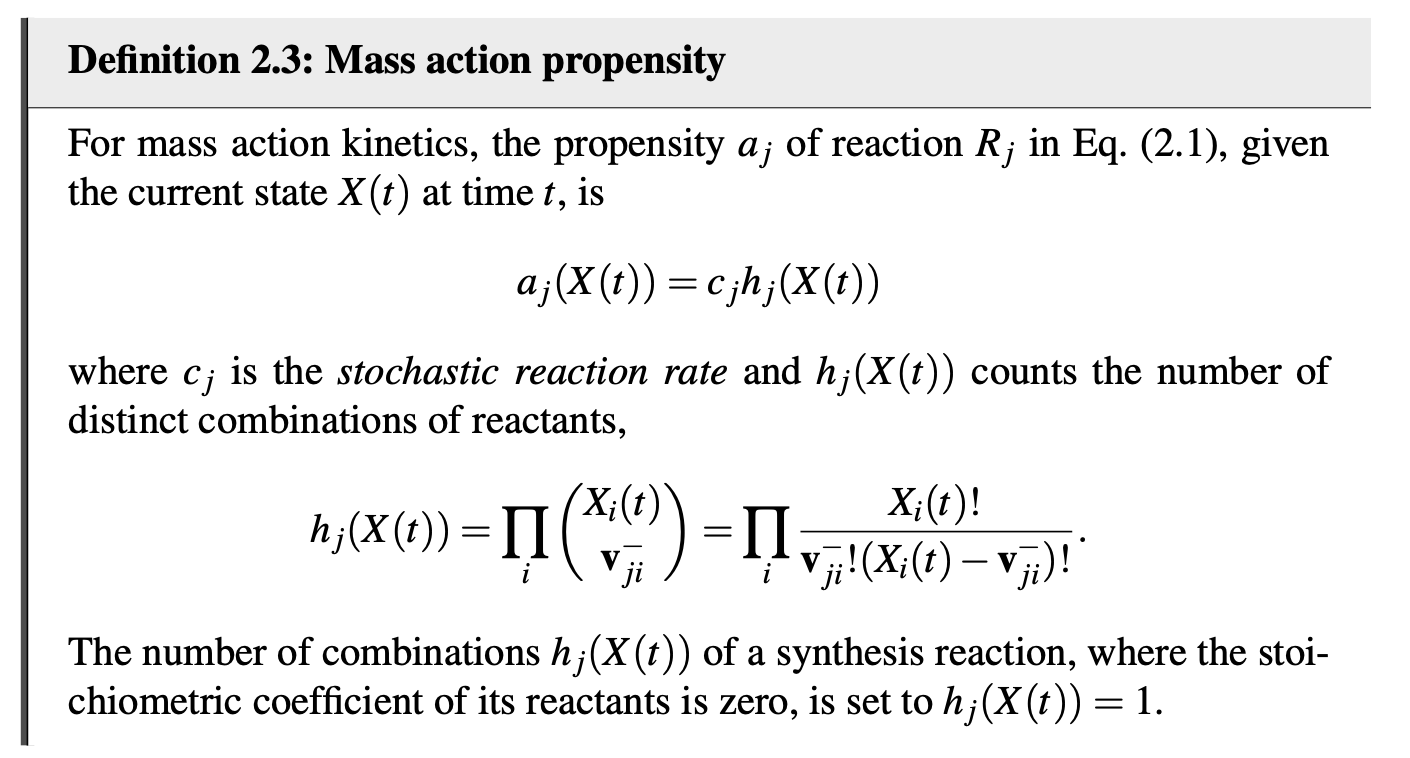
\includegraphics[width=0.5\textwidth]{massaction.png}
       \caption{Mass action propensity}
       \label{fig:massaction}
    \end{figure}

  \subsection{The propensity of a reaction}
  The propensity of a reaction is an intrinsic property of the reaction and is linked to the phenomenon that the reaction is going to represent.
  The probability will depend on the propensity of the reaction and the other reactions that are competing for the same reactant.
  The propensity is not affected by the products.

  $$a_1 (0) = c_1 h_1 (x(0))$$

  $$h_2(x(0)) = \begin{pmatrix}100 \\ 1 \end{pmatrix}\begin{pmatrix}50 \\ 1 \end{pmatrix}\begin{pmatrix}30 \\ 0 \end{pmatrix}$$

  $$x(0+ \tau) = x(0) + V_1 = \begin{bmatrix}99 &51& 30 \end{bmatrix}$$

  $$x(0) = \begin{bmatrix}100 &50& 30 \end{bmatrix}$$

  Since the combination is being computed $a^2$ will not be taken into account as in the canonical law of mass action.

    \subsubsection{Reaction propensity for reactions $ R_j$ with mass action kinetics}

    \begin{itemize}
      \item Synthesis reaction ($\emptyset$ → products): the number of combinations $ h_j = 1 $ and propensity $ a_j =c_j $
      \item Unimolecular reaction ($ S_i$ → products): the number of combinations $h_j= X_i$ and propensity $ a_j = c_jX_i $.
      \item Bimolecular reaction ($ S_i + S_k$ → products): the number of combinations $ h_j = X_iX_k$ and propensity $ a_j = c_jX_iX_k $.
      \item Dimerization reaction ($2S_i$ → products): the number of combinations $ h_j = \frac{1}{2}X_i(X_i -1) $ and propensity $ a_j = \frac{1}{2}c_jX_i(X_i -1) $.
      \item Polymerization reaction ($3S_i$ → products): the number of combinations $ h_j = 16X_i(X_i -1)(X_i -2)$ and propensity $ a_j = 16c_jX_i(X_i -1)(X_i -2) $.
      \item Termolecular reaction ($2S_i + S_k$ → products): the number of combinations $ h_j = \frac{1}{2}X_i(X_i -1)X_k$ and propensity $ a_j = \frac{1}{2}c_jX_i(X_i -1)X_k $.
    \end{itemize}


  \subsection{Chemical Master Equation}
  The CME is the theoretical approach allowing to derive the complete set of probabilities of all the possible states of the system.

    \subsubsection{Grand probability function}
    $\mathbb{P}\{\mathbf{x},t|\mathbf{x}_0,t_o\}$ is the probability that the system state is $X(t) = \mathbf{x}$ at time $t$, given the initial state $X(t_0) = \mathbf{x}_0$ at time $t_0$.
    By applying the chemical master equation, a set of differential equations for this probability is obtained, which theoretically provides the complete set of any of the states of the system.

    \subsubsection{CME}

    $$\frac{\mathbb{P}\{\mathbf{x},t|\mathbf{x}_0,t_o\}}{dt}= \sum_{j=1}^{M}(a_j(\mathbf{x}-\mathbf{v}_j)\mathbb{P}\{\mathbf{x},t|\mathbf{x}_0,t_o\})- \mathbb{P}\{\mathbf{x},t|\mathbf{x}_0,t_o\}\sum^M_{j=1}a_j(\mathbf{x})$$

    However, for computing all these probabilities in a complex system, the number of equations will increase and be practically useless.
    The idea is to avoid deriving everything with the chemical master equation but trying to apply another approach that is the one provided by the stochastic simulation.

\section{Stochastic simulation}
When applying the CME, all the possible state of the system are explored.
With a stochastic simulation only one possible trajectory of the system are computed (to obtain the total description many simulations have to be run).
The stochastic simulation works because only an idea of the most probable conditions of the system is needed.
A stochastic simulation is faster than a real experiment and it can be run on a personal computer (also thousands of simulations can be performed).

  \subsection{Probability density function}
  The mathematical basis of a stochastic simulation is the reaction probability density function (pdf).
  $p(\tau, \mu |\mathbf{x}, t)d\tau$ is the probability that a reaction $R_\mu$ fires in the next infinitesimal time interval $[t+\tau,t+\tau+d\tau)$, given the state $X(t) = \mathbf{x}$ at time $t$.
  \\
  \\
  \noindent

    \subsubsection{Computing the probability density function}
    These probabilities can be computed by considering the idea of propensity.
    The propensity is a formula on the state of the system which depends on some of the variables that are in the system that allows to provide a quantitative information that can be used to derive the probabilities.
    The propensity is not a probability: propensity is not in a range from $0$ to $1$ and it is a property of a reaction while the probability is a property of the system.
    One of the crucial points of a stochastic simulation is that there is a need to be able to sample from this probability distribution  function given the fact that the computer has few ways of generating something that is stochastic.
    The easiest way to do so is through a random number generator.
    The pseudocode in figure \ref{fig:SSA} implements this procedure.

    \begin{figure}
      \centering
      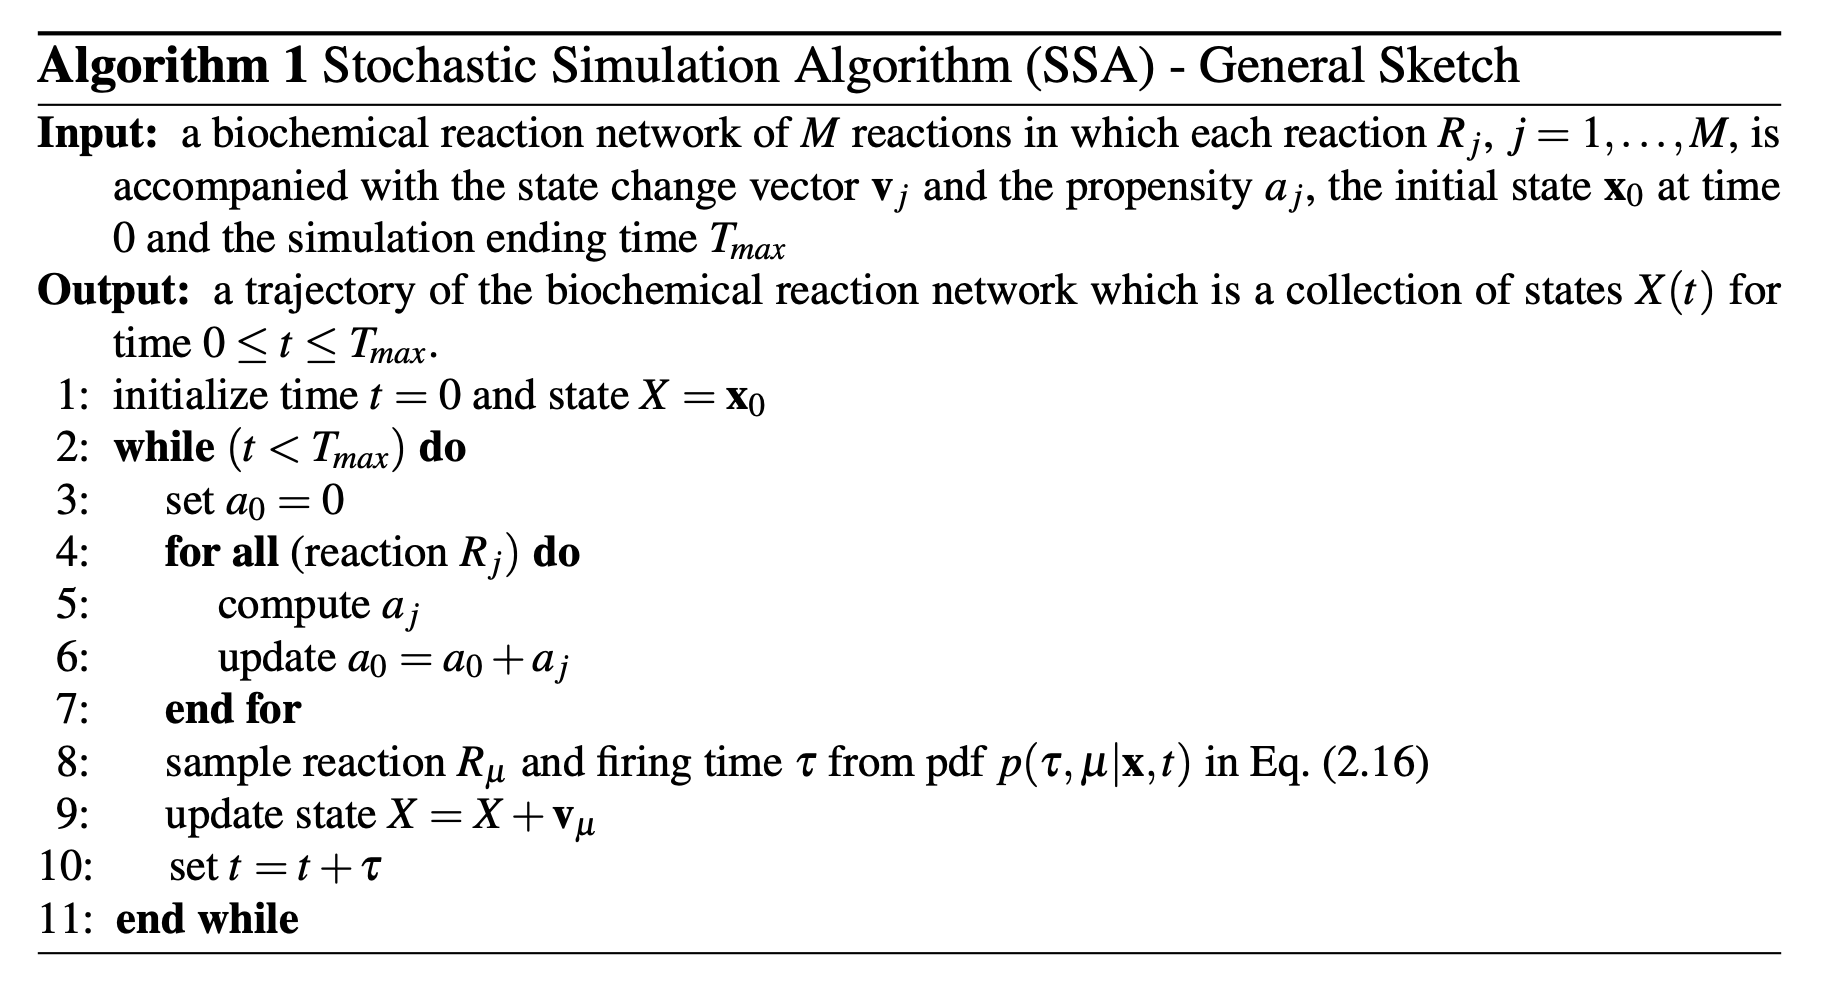
\includegraphics[width=\textwidth]{SSA_algo.png}
      \caption{SSA}
      \label{fig:SSA}
    \end{figure}

    The result of a SSA run is a \emph{trajectory}, which shows the evolution of the biological system over time.
    The trajectory is a collection of states $\emph{X}(\emph{t})$ that denotes the state of the system at any time $0 \leq \emph{t}\geq \emph{Tmax}$.
    It should be emphasized that because SSA is a discrete event simulation algorithm, the state changes only at discrete time instants when reactions fire.
    The state between two reaction firings is a constant.
